\documentclass[ucs, notheorems, handout]{beamer}

\usetheme[numbers,totalnumbers,compress, nologo]{Statmod}
\usefonttheme[onlymath]{serif}
\setbeamertemplate{navigation symbols}{}

%\mode<handout> {
%    \usepackage{pgfpages}
%    \setbeameroption{show notes}
%    \pgfpagesuselayout{2 on 1}[a4paper, border shrink=5mm]
%    \setbeamercolor{note page}{bg=white}
%    \setbeamercolor{note title}{bg=gray!10}
%    \setbeamercolor{note date}{fg=gray!10}
%}

\usepackage[utf8x]{inputenc}
\usepackage[T2A]{fontenc}
\usepackage[english, russian]{babel}
\usepackage{amsmath}
\usepackage{amsfonts}
\usepackage{tikz}
\usepackage{ragged2e}
\usepackage{wrapfig}
\usepackage{t-angles}
\usepackage{slashbox}
\usepackage{hhline}
\usepackage{multirow}
\usepackage{graphics}
\usepackage{color}
\usepackage{mathdots}
\usepackage{graphicx}
\usepackage{mdwtab}
%new calligraphic font for subspaces 
\usepackage{euscript}
\newcommand{\cA}{\EuScript{A}}
\newcommand{\cB}{\EuScript{B}}
\newcommand{\cC}{\EuScript{C}}
\newcommand{\cD}{\EuScript{D}}
\newcommand{\cE}{\EuScript{E}}
\newcommand{\cF}{\EuScript{F}}
\newcommand{\cG}{\EuScript{G}}
\newcommand{\cH}{\EuScript{H}}
\newcommand{\cI}{\EuScript{I}}
\newcommand{\cJ}{\EuScript{J}}
\newcommand{\cK}{\EuScript{K}}
\newcommand{\cL}{\EuScript{L}}
\newcommand{\cM}{\EuScript{M}}
\newcommand{\cN}{\EuScript{N}}
\newcommand{\cO}{\EuScript{O}}
\newcommand{\cP}{\EuScript{P}}
\newcommand{\cQ}{\EuScript{Q}}
\newcommand{\cR}{\EuScript{R}}
\newcommand{\cS}{\EuScript{S}}
\newcommand{\cT}{\EuScript{T}}
\newcommand{\cU}{\EuScript{U}}
\newcommand{\cV}{\EuScript{V}}
\newcommand{\cW}{\EuScript{W}}
\newcommand{\cX}{\EuScript{X}}
\newcommand{\cY}{\EuScript{Y}}
\newcommand{\cZ}{\EuScript{Z}}

%font for text indices like transposition X^\mathrm{T}
\newcommand{\rmA}{\mathrm{A}}
\newcommand{\rmB}{\mathrm{B}}
\newcommand{\rmC}{\mathrm{C}}
\newcommand{\rmD}{\mathrm{D}}
\newcommand{\rmE}{\mathrm{E}}
\newcommand{\rmF}{\mathrm{F}}
\newcommand{\rmG}{\mathrm{G}}
\newcommand{\rmH}{\mathrm{H}}
\newcommand{\rmI}{\mathrm{I}}
\newcommand{\rmJ}{\mathrm{J}}
\newcommand{\rmK}{\mathrm{K}}
\newcommand{\rmL}{\mathrm{L}}
\newcommand{\rmM}{\mathrm{M}}
\newcommand{\rmN}{\mathrm{N}}
\newcommand{\rmO}{\mathrm{O}}
\newcommand{\rmP}{\mathrm{P}}
\newcommand{\rmQ}{\mathrm{Q}}
\newcommand{\rmR}{\mathrm{R}}
\newcommand{\rmS}{\mathrm{S}}
\newcommand{\rmT}{\mathrm{T}}
\newcommand{\rmU}{\mathrm{U}}
\newcommand{\rmV}{\mathrm{V}}
\newcommand{\rmW}{\mathrm{W}}
\newcommand{\rmX}{\mathrm{X}}
\newcommand{\rmY}{\mathrm{Y}}
\newcommand{\rmZ}{\mathrm{Z}}

%tt font for time series
\newcommand{\tA}{\mathsf{A}}
\newcommand{\tB}{\mathsf{B}}
\newcommand{\tC}{\mathsf{C}}
\newcommand{\tD}{\mathsf{D}}
\newcommand{\tE}{\mathsf{E}}
\newcommand{\tF}{\mathsf{F}}
\newcommand{\tG}{\mathsf{G}}
\newcommand{\tH}{\mathsf{H}}
\newcommand{\tI}{\mathsf{I}}
\newcommand{\tJ}{\mathsf{J}}
\newcommand{\tK}{\mathsf{K}}
\newcommand{\tL}{\mathsf{L}}
\newcommand{\tM}{\mathsf{M}}
\newcommand{\tN}{\mathsf{N}}
\newcommand{\tO}{\mathsf{O}}
\newcommand{\tP}{\mathsf{P}}
\newcommand{\tQ}{\mathsf{Q}}
\newcommand{\tR}{\mathsf{R}}
\newcommand{\tS}{\mathsf{S}}
\newcommand{\tT}{\mathsf{T}}
\newcommand{\tU}{\mathsf{U}}
\newcommand{\tV}{\mathsf{V}}
\newcommand{\tW}{\mathsf{W}}
\newcommand{\tX}{\mathsf{X}}
\newcommand{\tY}{\mathsf{Y}}
\newcommand{\tZ}{\mathsf{Z}}

%bf font for matrices
\newcommand{\bfA}{\mathbf{A}}
\newcommand{\bfB}{\mathbf{B}}
\newcommand{\bfC}{\mathbf{C}}
\newcommand{\bfD}{\mathbf{D}}
\newcommand{\bfE}{\mathbf{E}}
\newcommand{\bfF}{\mathbf{F}}
\newcommand{\bfG}{\mathbf{G}}
\newcommand{\bfH}{\mathbf{H}}
\newcommand{\bfI}{\mathbf{I}}
\newcommand{\bfJ}{\mathbf{J}}
\newcommand{\bfK}{\mathbf{K}}
\newcommand{\bfL}{\mathbf{L}}
\newcommand{\bfM}{\mathbf{M}}
\newcommand{\bfN}{\mathbf{N}}
\newcommand{\bfO}{\mathbf{O}}
\newcommand{\bfP}{\mathbf{P}}
\newcommand{\bfQ}{\mathbf{Q}}
\newcommand{\bfR}{\mathbf{R}}
\newcommand{\bfS}{\mathbf{S}}
\newcommand{\bfT}{\mathbf{T}}
\newcommand{\bfU}{\mathbf{U}}
\newcommand{\bfV}{\mathbf{V}}
\newcommand{\bfW}{\mathbf{W}}
\newcommand{\bfX}{\mathbf{X}}
\newcommand{\bfY}{\mathbf{Y}}
\newcommand{\bfZ}{\mathbf{Z}}

%bb font for standard spaces and expectation
\newcommand{\bbA}{\mathbb{A}}
\newcommand{\bbB}{\mathbb{B}}
\newcommand{\bbC}{\mathbb{C}}
\newcommand{\bbD}{\mathbb{D}}
\newcommand{\bbE}{\mathbb{E}}
\newcommand{\bbF}{\mathbb{F}}
\newcommand{\bbG}{\mathbb{G}}
\newcommand{\bbH}{\mathbb{H}}
\newcommand{\bbI}{\mathbb{I}}
\newcommand{\bbJ}{\mathbb{J}}
\newcommand{\bbK}{\mathbb{K}}
\newcommand{\bbL}{\mathbb{L}}
\newcommand{\bbM}{\mathbb{M}}
\newcommand{\bbN}{\mathbb{N}}
\newcommand{\bbO}{\mathbb{O}}
\newcommand{\bbP}{\mathbb{P}}
\newcommand{\bbQ}{\mathbb{Q}}
\newcommand{\bbR}{\mathbb{R}}
\newcommand{\bbS}{\mathbb{S}}
\newcommand{\bbT}{\mathbb{T}}
\newcommand{\bbU}{\mathbb{U}}
\newcommand{\bbV}{\mathbb{V}}
\newcommand{\bbW}{\mathbb{W}}
\newcommand{\bbX}{\mathbb{X}}
\newcommand{\bbY}{\mathbb{Y}}
\newcommand{\bbZ}{\mathbb{Z}}

%got font for any case
\newcommand{\gA}{\mathfrak{A}}
\newcommand{\gB}{\mathfrak{B}}
\newcommand{\gC}{\mathfrak{C}}
\newcommand{\gD}{\mathfrak{D}}
\newcommand{\gE}{\mathfrak{E}}
\newcommand{\gF}{\mathfrak{F}}
\newcommand{\gG}{\mathfrak{G}}
\newcommand{\gH}{\mathfrak{H}}
\newcommand{\gI}{\mathfrak{I}}
\newcommand{\gJ}{\mathfrak{J}}
\newcommand{\gK}{\mathfrak{K}}
\newcommand{\gL}{\mathfrak{L}}
\newcommand{\gM}{\mathfrak{M}}
\newcommand{\gN}{\mathfrak{N}}
\newcommand{\gO}{\mathfrak{O}}
\newcommand{\gP}{\mathfrak{P}}
\newcommand{\gQ}{\mathfrak{Q}}
\newcommand{\gR}{\mathfrak{R}}
\newcommand{\gS}{\mathfrak{S}}
\newcommand{\gT}{\mathfrak{T}}
\newcommand{\gU}{\mathfrak{U}}
\newcommand{\gV}{\mathfrak{V}}
\newcommand{\gW}{\mathfrak{W}}
\newcommand{\gX}{\mathfrak{X}}
\newcommand{\gY}{\mathfrak{Y}}
\newcommand{\gZ}{\mathfrak{Z}}

%old calligraphic font
\newcommand{\calA}{\mathcal{A}}
\newcommand{\calB}{\mathcal{B}}
\newcommand{\calC}{\mathcal{C}}
\newcommand{\calD}{\mathcal{D}}
\newcommand{\calE}{\mathcal{E}}
\newcommand{\calF}{\mathcal{F}}
\newcommand{\calG}{\mathcal{G}}
\newcommand{\calH}{\mathcal{H}}
\newcommand{\calI}{\mathcal{I}}
\newcommand{\calJ}{\mathcal{J}}
\newcommand{\calK}{\mathcal{K}}
\newcommand{\calL}{\mathcal{L}}
\newcommand{\calM}{\mathcal{M}}
\newcommand{\calN}{\mathcal{N}}
\newcommand{\calO}{\mathcal{O}}
\newcommand{\calP}{\mathcal{P}}
\newcommand{\calQ}{\mathcal{Q}}
\newcommand{\calR}{\mathcal{R}}
\newcommand{\calS}{\mathcal{S}}
\newcommand{\calT}{\mathcal{T}}
\newcommand{\calU}{\mathcal{U}}
\newcommand{\calV}{\mathcal{V}}
\newcommand{\calW}{\mathcal{W}}
\newcommand{\calX}{\mathcal{X}}
\newcommand{\calY}{\mathcal{Y}}
\newcommand{\calZ}{\mathcal{Z}}


\setbeamercolor{bluetext_color}{fg=blue}
\newcommand{\bluetext}[1]{{\usebeamercolor[fg]{bluetext_color}#1}}

\newtheorem{theorem}{Теорема}
\newtheorem{statement}{Утверждение}

\title[HO-MSSA]{High-order MSSA для выделения сигнала}

\author[Хромов Н.А., Голяндина Н.Э.]{Хромов Никита Андреевич, Голяндина Нина Эдуардовна}

\institute[Санкт-Петербургский Государственный Университет]{%
    \small
    Санкт-Петербургский государственный университет\\
    Кафедра статистического моделирования\\
    \vspace{1.6cm}
}

\date{Процессы управления и устойчивость\\
2 апреля 2024, Санкт-Петербург}

\subject{Talks}

\begin{document}

    \begin{frame}[plain]
        \titlepage

    \end{frame}


    \section{Введение}\label{sec:introduction}
    \begin{frame}{Постановка задачи}
        $\tX=(x_0, x_1,\ldots, x_{N-1})$, $x_i\in \mathbb{R}$ "--- вещественный временной ряд.

        $\tX = \tT + \tP + \tR$.

        $\tT$ "--- тренд, $\tP$ "--- регулярные колебания, $\tR$ "--- шум.
        \vspace{0.3cm}

        \bluetext{Возможные задачи:}
        \begin{enumerate}
            \item Выделение сигнала из ряда: нахождение $\tS = \tT + \tP$,
            \item Отделение компонент сигнала: нахождение $\tT$ и $\tP$,
            \item Нахождение параметров сигнала в параметрической модели.
        \end{enumerate}

        \vspace{0.3cm}
        Методы, основанные на подпространстве сигнала:
        \begin{itemize}
            \item SSA (задачи 1 и 2)
            \\(Golyandina et al.\ (2001), Analysis of time series structure: SSA and related techiques)
            \item ESPRIT (задача 3)
            \\(Roy, Kailath (1989), ESPRIT-estimation of signal parameters via rotational invariance techniques)
        \end{itemize}
    \end{frame}

    \begin{frame}{Пример применения SSA и ESPRIT}
        \[
            s_n = e^{-0.01 n} \cos(2\pi n / 3) + e^{-0.02 n} \cos(2\pi n / 4), \quad n=0, 1, \ldots, 46
        \]

        \smallskip
        \center
        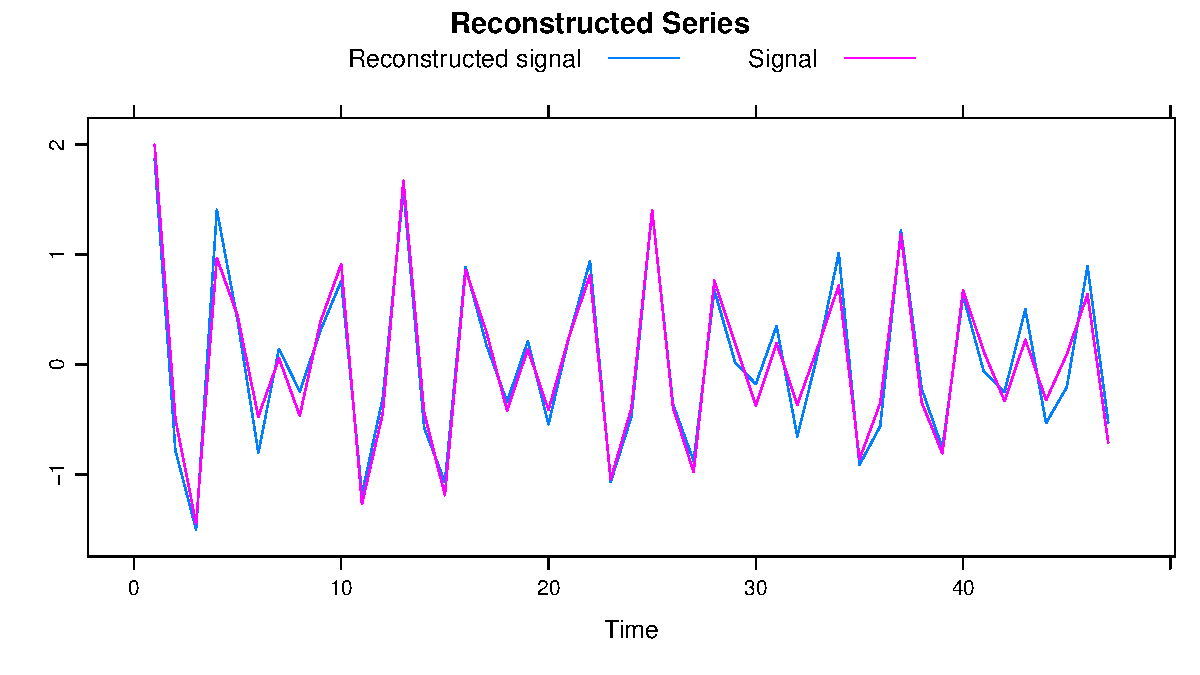
\includegraphics[width=\textwidth]{img/decomp}
    \end{frame}

    \begin{frame}{Пример применения SSA и ESPRIT}
        \begin{center}
            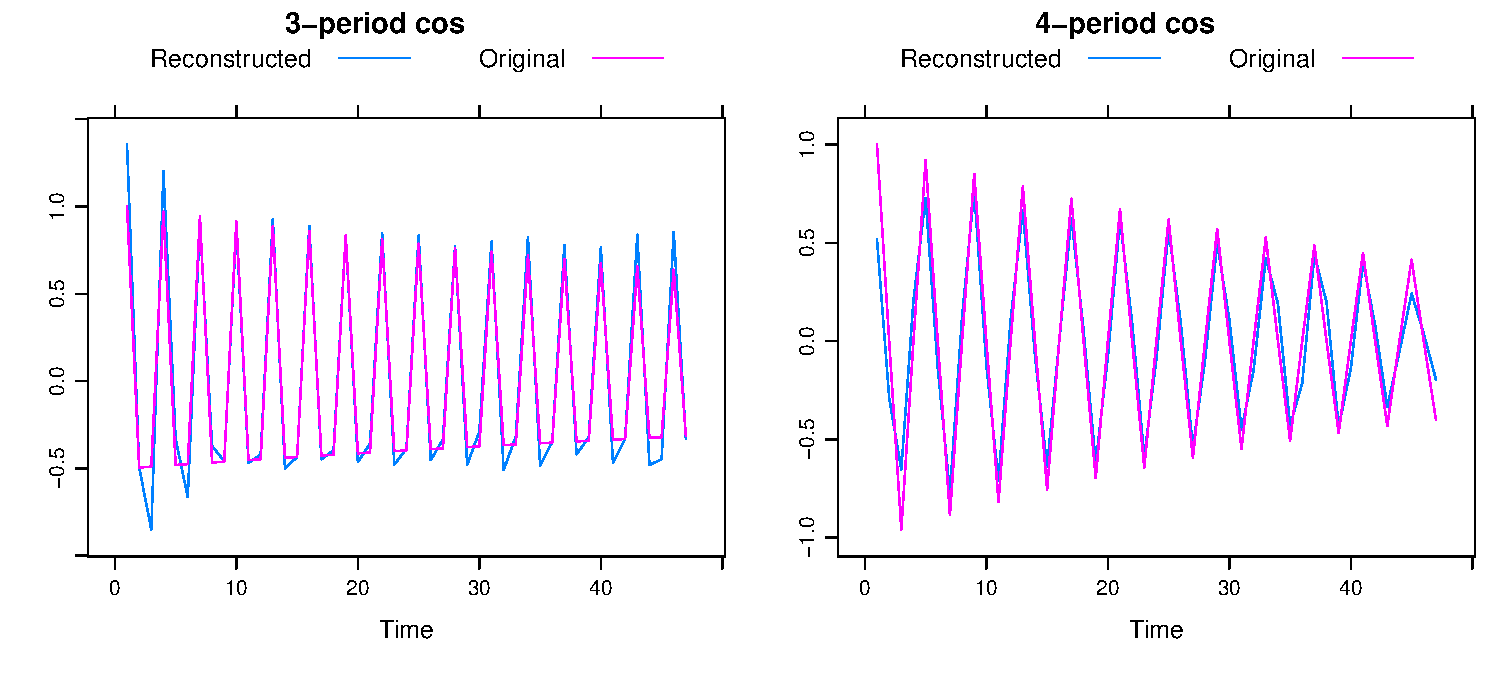
\includegraphics[width=\textwidth]{img/rec}
        \end{center}
%        Восстановленные ESPRIT параметры
        \begin{table}
            \caption{Восстановленные ESPRIT параметры}
            \begin{tabular}{|c|c|c|}
                \hline
                Номер слагаемого  & 1         & 2        \\ \hline
                Период            & $3$       & $4.06$   \\ \hline
                Степень затухания & $ -0.008$ & $-0.027$ \\ \hline
            \end{tabular}
        \end{table}
%        \begin{itemize}
%            \item \bluetext{Периоды}: $T_1 = 3$, $T_2 = 4.06$
%            \item \bluetext{Степени затухания}: $\alpha_1 = -0.008$, $\alpha_2 = -0.027$
%        \end{itemize}

    \end{frame}

    \begin{frame}{Постановка задачи}
        В работе Papy et al.\ (2005) была предложена тензорная модификация метода ESPRIT и экспериментально показано её
        преимущество для конкретной модели.

        \medskip

        \textcolor{red}{Цель:} расширение предложенного Papy алгоритма для решения задачи выделения сигнала,
        исследование свойств тензорных модификаций методов семейства SSA с точки зрения
        точности выделения сигнала.

        \smallskip

        В докладе рассмотрена тензорная модификация для выделения сигнала из многомерных временных рядов.
    \end{frame}


    \section{Модель}\label{sec:model}
    \begin{frame}{Модель одномерного сигнала}
        $\tX = (x_0, x_1, \ldots, x_{N-1}) = \tS + \tR$,\\
        $\tS$ --- сигнал, $\tR$ --- шум.

        \vspace{0.4cm}

        \[
            s_n = \sum_{j=1}^{R} a_j e^{ -\alpha_j n }
            \cos\left( 2 \pi \omega_j n + \varphi_j\right)
        \]

        \vspace{0.3cm}
        Параметры:\\
        $a_j \in \mathbb{R}\setminus\{0\}$ --- амплитуды, $\alpha_j \in \mathbb{R}$ --- степени затухания,
        $\omega_j \in [0, 1/2]$ --- частоты, $\varphi_j \in [0, 2\pi)$ --- фазы.

    \end{frame}

    \begin{frame}{Модель многомерного сигнала}
%        $\tX =
%        \begin{pmatrix}
%            \tX_1\\
%            \tX_2\\
%            \vdots\\
%            \tX_P
%        \end{pmatrix}
%        =
%        \begin{pmatrix}
%            \tS_1\\
%            \tS_2\\
%            \vdots\\
%            \tS_P
%        \end{pmatrix} +
%        \begin{pmatrix}
%            \tR_1\\
%            \tR_2\\
%            \vdots\\
%            \tR_P
%        \end{pmatrix} = \tS + \tR
%        $.
        $\tX =
        \begin{pmatrix}
            \tX_1  \\
            \tX_2  \\
            \vdots \\
            \tX_P
        \end{pmatrix}
        $, $\quad\tX_p = \tS_p + \tR_p$ --- одномерные ряды.

        \vspace{0.4cm}
        Общий случай:
        \[
            s_n^{(p)} = \sum_{j=1}^{R(p)} a_j^{(p)} e^{ -\alpha_j^{(p)} n }
            \cos\left( 2 \pi \omega_j^{(p)} n + \varphi_j^{(p)}\right)
        \]
        Рассматриваемый случай:
        \[
            s_n^{(p)} = \sum_{j=1}^{R} a_j^{(p)} e^{ -\alpha_j n }
            \cos\left( 2 \pi \omega_j n + \varphi_j^{(p)}\right)
        \]
    \end{frame}


    \section{MSSA}\label{sec:mssa}
    \begin{frame}{Описание алгоритма MSSA}
        $\tX$ --- $P$-мерный временной ряд длины $N$ с сигналом $\tS$, $L$ --- длина окна,
        $K = N - L + 1$.

        \vspace{0.5cm}

        \bluetext{Оператор вложения одномерного ряда:}
        \[
            \mathbb{H}_L\left( \tX_p \right) =
            \begin{pmatrix}
                x_0^{(p)}     & x_1^{(p)} & { x}_2^{(p)} & \ldots        & x_{K-1}^{(p)} \\
                x_1^{(p)}     & x_2^{(p)} & \iddots      & \ldots        & \vdots        \\
                x_2^{(p)}     & \iddots   & \iddots      & \ldots        & \vdots        \\
                \vdots        & \vdots    & \vdots       & \vdots        & x_{N-2}^{(p)} \\
                x_{L-1}^{(p)} & \ldots    & \ldots       & x_{N-2}^{(p)} & x_{N-1}^{(p)} \\
            \end{pmatrix}
        \]
    \end{frame}

    \begin{frame}{Описание алгоритма MSSA}
        \bluetext{Параметры алгоритма:} $L,\, R:\: R \leqslant L < N,\, K \geqslant L$.\\
        $R$ --- число компонент, отнесённых к сигналу.

        \vspace{0.3cm}

        \bluetext{Схема алгоритма MSSA для выделения сигнала}
        \begin{enumerate}
            \item \bluetext{Вложение} $\tX \stackrel{\textcolor{red}{L}}{\mapsto} \bfH =
            [\bbH_L(\tX_1):\bbH_L(\tX_2): \dots: \bbH_L(\tX_P)]\in \bbR^{L\times KP},$

            \vspace{0.2cm}

            \item \bluetext{Разложение} $\bfH = \sum_{i=1}^{d} \sqrt{\lambda_i}U_i V_i^\rmT,\,\, d \leqslant L$

            \vspace{0.2cm}

            \item \bluetext{Группировка} $\tilde{\bfS}= \sum_{i=1}^{\textcolor{red}{R}} \sqrt{\lambda_i}U_i V_i^\rmT,\,\,
            R \leqslant d$

            \vspace{0.2cm}

            $\tilde{\bfS} = \left[ \tilde{\bfS}_1 : \tilde{\bfS}_2 : \cdots : \tilde{\bfS}_P \right]$,
            $\quad \tilde{\bfS}_p \in \bbR^{L\times K}$

            \vspace{0.2cm}

            \item \bluetext{Восстановление} Матрицы $\tilde{\bfS}_p$ усредняются вдоль побочных диагоналей:
            $\tilde{s}_n^{(p)} = \operatorname{mean}\left\{\left(\tilde{\bfS}_p\right)_{i,j}~\middle|~i + j - 2 = n\right\}.$
        \end{enumerate}
    \end{frame}

    \begin{frame}{Ранг сигнала}
        $\tS$ имеет ранг $r$, если $\forall L:~r \leqslant \min(L, K) \,\,\, \operatorname{rank}{\bbH_L(\tS)} = r$.

        Рекомендуемый выбор параметра $R$ в алгоритме: $R=r$.

        \vspace{0.4cm}

        \bluetext{Примеры}
        \begin{itemize}
            \item $s_n = A e^{\alpha n} \cos(2\pi \omega n + \varphi),$\\
            $A \ne 0,\, \alpha \in \bbR,\, \omega \in [0, 1/2],\, \varphi \in [0, 2\pi)$
            \[
                r(\omega) =
                \begin{cases}
                    1, & \omega \in \{0, 1/2\},\\
                    2, & \omega \in (0, 1/2).
                \end{cases}
            \]
            \item
            \[
                s_n^{(p)} = \sum_{j=1}^{R} a_j^{(p)} e^{ -\alpha_j n }
                \cos\left( 2 \pi \omega_j n + \varphi_j^{(p)}\right)
            \]
            $\displaystyle r = \sum_{(\omega, \alpha) \in \Omega} r(\omega)$, $\quad \Omega$ --- все уникальные пары $(\omega_j, \alpha_j)$.
        \end{itemize}
    \end{frame}


    \section{High-Order MSSA}\label{sec:high-order-mssa}
    \begin{frame}{Построение траекторного тензора}
        \center
        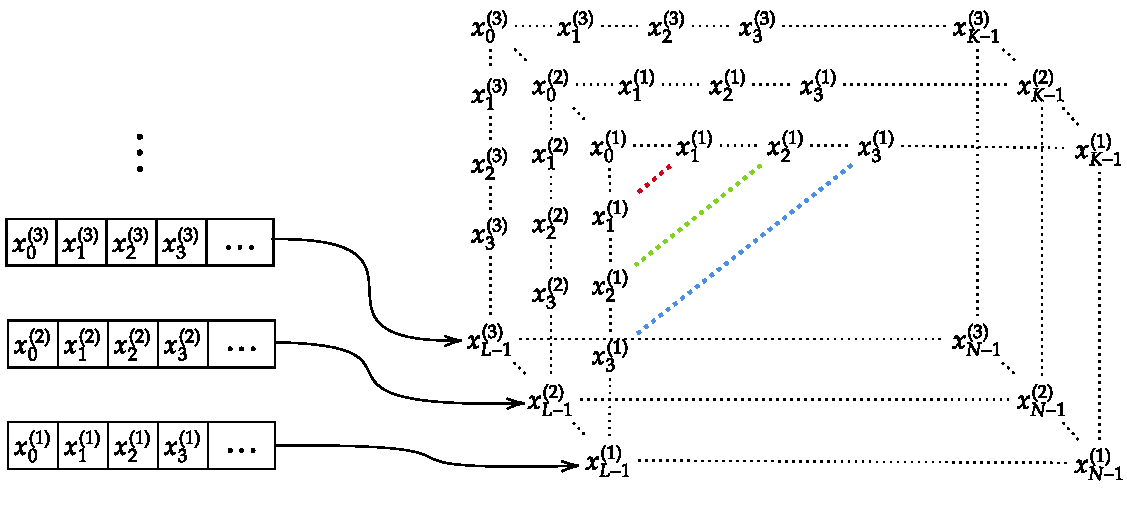
\includegraphics[width=\textwidth]{img/mssa-tensor-injection}

        $L < N$, $\quad K = N - L + 1 \geqslant L$
    \end{frame}

    \begin{frame}{Разложение и группировка}
        \begin{itemize}
            \item High-Order SVD траекторного тензора $\calH$ имеет вид
            \[
                \calH = \sum_{l=1}^{L} \sum_{k=1}^{K} \sum_{p=1}^{P} c_{lkp} \mathbf{U}^{(1)}_{l}
                \circ \mathbf{U}^{(2)}_{k} \circ \mathbf{U}^{(3)}_{p}.
            \]

            \vspace{0.4cm}
            \item Этап группировки в алгоритме HO-MSSA имеет вид
            \[
                \widetilde{\calH} = \sum_{l=1}^{R_1} \sum_{k=1}^{R_2} \sum_{p=1}^{R_3} c_{lkp} \mathbf{U}^{(1)}_{l}
                \circ \mathbf{U}^{(2)}_{k} \circ \mathbf{U}^{(3)}_{p},
            \]
            $R_i\leqslant \min(L, K, P)$ --- параметры алгоритма.
        \end{itemize}
    \end{frame}


    \section{Ранги сигнала в HO-MSSA}\label{sec:tensor-ranks}
    \begin{frame}{Ранги тензора}
        \bluetext{$n$-Ранг тензора:} размерность пространства, порождённого
        векторами вдоль $n$-го измерения ($\operatorname{rank}_n(\mathcal{A})$).

        \begin{theorem}
            Пусть многомерный временной ряд
            \[
                \left( x_0^{(p)}, x_1^{(p)}, \ldots, x_{N-1}^{(p)} \right), \quad p=1, 2,\ldots, P
            \]
            имеет ранг $d$ в терминах MSSA, тогда для траекторного тензора $\mathcal{H}$, построенного по любой длине окна $L<N$
            такой, что ${\min(L, K) \geqslant d}$, выполняется $\operatorname{rank}_1(\mathcal{H})=\operatorname{rank}_2(\mathcal{H})=d$,
            а $3$-ранг этого тензора равен рангу матрицы, в строках которой записаны заданные одномерные ряды.
        \end{theorem}
    \end{frame}

    \begin{frame}{Ранги сигнала в HO-MSSA}
        \begin{itemize}
            \item $1$- и $2$-ранги траекторного тензора $\calH$ сигнала $\tS$ совпадают с рангом этого сигнала в терминах MSSA.
            \item Однако ранг третьего измерения имеет иной смысл.
        \end{itemize}

        \vspace{0.2cm}

        На этапе группировки рекомендуется брать $R_1=R_2=r$ и $R_3 = r_3$, где $r$ --- MSSA-ранг сигнала,
        $r_3$ --- ранг матрицы, составленной из $\tS_p$.

        \vspace{0.2cm}

        \bluetext{Примеры}
        \[
            s_n^{(p)} = \sum_{j=1}^{R} a_j^{(p)} e^{ -\alpha_j n }\cos\left( 2 \pi \omega_j n + \varphi_j^{(p)}\right),
            \quad n\in \overline{0:N-1},
        \]
        $p\in \overline{1:P},\, a_j^{(p)}\ne 0,\, \alpha_j \in \bbR,\, \omega_j \in(0, 1/2),\, \varphi_j^{(p)}\in [0, 2\pi)$

        \vspace{0.1cm}

        \begin{enumerate}
            \item $\omega_i \ne \omega_j,\, \varphi_j^{(p)} = \varphi_j^{(m)} \hspace{0.53cm}
            \implies r = 2R,\, r_3 = R$,
            \item $\omega_i \ne \omega_j,\, \varphi_j^{(p)} = b_j p+c_j
            \implies r = 2R,\, r_3 = 2R$.
        \end{enumerate}
    \end{frame}


    \section{Численные сравнения}\label{sec:numerical-comparisons}
    \begin{frame}{Численные сравнения}
        \begin{enumerate}
            \item \bluetext{Одинаковые фазы}
            \[
                x_n^{(p)} = c_1^{(p)} e^{-0.01 n} \cos(2\pi 0.2 n) + c_2^{(p)} e^{-0.02 n} \cos(2\pi 0.22 n) + \varepsilon_n^{(p)},
            \]
            \item \bluetext{Линейно меняющиеся фазы}
            \[
                \begin{split}
                    x_n^{(p)} &= c_1^{(p)} e^{-0.01 n} \cos(2\pi 0.2 n + p \pi / 6)\\
                    &+ c_2^{(p)} e^{-0.02 n} \cos(2\pi 0.22 n + p \pi / 9) + \varepsilon_n^{(p)},
                \end{split}
            \]
        \end{enumerate}
        В обоих случаях $n=0,1,\ldots, 24$, $p=1,2,\ldots, 12$, $c_k^{(p)}\sim \rmN(0, 1)$, $\varepsilon_n^{(p)}\sim \rmN(0, 0.02)$
        и независимы.

        \vspace{0.2cm}
        Точность сравнивалась по RMSE по 1000 реализациям шума $\varepsilon_n^{(p)}$ при фиксированных $c_k^{(p)}$,
        сравнение проводилось на одних и тех же реализациях шума при выборе оптимальных
        для каждого метода параметров $L$, $R$ и $R_3$.
    \end{frame}

    \begin{frame}{Численные сравнения}
        \begin{enumerate}
            \item Равные фазы \\
            \bluetext{MSSA}: $L = 22$, $R=4$\\
            \bluetext{HO-MSSA}: $L = 20$, $R=4$, $R_3=2$
            \item Линейно меняющиеся фазы\\
            \bluetext{MSSA}: $L = 21$, $R=4$\\
            \bluetext{HO-MSSA}: $L = 21$, $R=4$, $R_3=4$
        \end{enumerate}

        \vspace{-0.4cm}
        \begin{table}[!ht]
            \centering
            \caption{RMSE оценки многомерного сигнала}
            \begin{tabular}{|l|c|c|}
                \hline
                & MSSA      & HO-MSSA   \\ \hline
                равные фазы   & $0.0107$  & $0.0079$  \\ \hline
                линейные фазы & $0.00924$ & $0.00918$ \\ \hline
            \end{tabular}
        \end{table}

        \vspace{0.2cm}
        \textcolor{red}{Вывод}: HO-MSSA выделяет многомерный сигнал с одной частотой точнее, чем MSSA.
    \end{frame}


%    \section{Выводы}\label{sec:conclusion}
%    \begin{frame}{Выводы}
%        \begin{itemize}
%            \item Тензорный вариант HO-MSSA для выделения многомерного сигнала дал точность выше, чем обычный MSSA.
%            \item
%        \end{itemize}
%    \end{frame}
\end{document}
